% Phase-6 reproducible, non-quantitative evaluation-sequence diagram.
\documentclass[border=0pt]{standalone}
\usepackage[T1]{fontenc}
\usepackage{mathptmx}
\usepackage{tikz}
\usetikzlibrary{arrows.meta}
\pdfinfoomitdate=1
\pdftrailerid{}
\pdfsuppressptexinfo=15
\definecolor{ink}{HTML}{24313D}
\definecolor{accent}{HTML}{366D95}
\definecolor{pale}{HTML}{F2F5F7}
\begin{document}
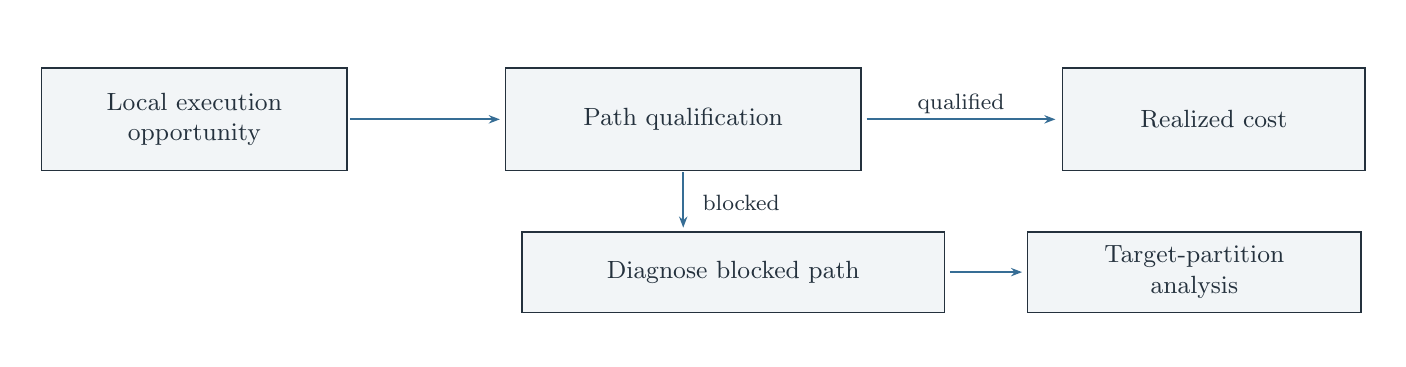
\begin{tikzpicture}[x=1bp,y=-1bp,inner sep=0,outer sep=0,text=ink]
\path[use as bounding box] (0,0) rectangle (486,112);
\tikzset{stagebox/.style={draw=ink,line width=.55bp,fill=pale,align=center,font=\fontsize{9}{11}\selectfont},
         flow/.style={-{Stealth[length=4bp,width=3bp]},line width=.7bp,draw=accent},
         flowlabel/.style={font=\fontsize{8}{9.5}\selectfont,align=center}}
\node[stagebox,minimum width=110bp,minimum height=37bp] at (60,33) {Local execution\\opportunity};
\node[stagebox,minimum width=128bp,minimum height=37bp] at (236,33) {Path qualification};
\node[stagebox,minimum width=109bp,minimum height=37bp] at (427,33) {Realized cost};
\draw[flow] (116,33) -- (170,33);
\draw[flow] (302,33) -- (370,33);
\node[flowlabel,anchor=south] at (336,31) {qualified};
\node[stagebox,minimum width=152bp,minimum height=29bp] at (254,88) {Diagnose blocked path};
\node[stagebox,minimum width=120bp,minimum height=29bp] at (420,88) {Target-partition\\analysis};
\draw[flow] (236,52) -- (236,72);
\node[flowlabel,anchor=west] at (243,63) {blocked};
\draw[flow] (332,88) -- (358,88);
\end{tikzpicture}
\end{document}
